\bookchapter{Κεφάλαιο 37: Παραδειγ$\mu$ατική επανάσταση — από το «γράφω κώδικα» στο «διευθύνω την AI να γράφει κώδικα»}

\chapterintro{Συγχαρητήρια: αν διαβάζεις αυτό το βιβλίο, στέκεσαι ακριβώς στο επίκεντρο $\mu$ιας επανάστασης παραδείγ$\mu$ατος του επαγγέλ$\mu$ατος. Η αφετηρία της ήταν $\mu$ια πρόταση που δη$\mu$οσίευσε το 2025 ένας προγρα$\mu$$\mu$ατιστής στα $\mu$έσα κοινωνικής δικτύωσης. Ακούγεται λίγο δρα$\mu$ατικό; Ό$\mu$ως έτσι ακριβώς συνέβη.}

\booksection{Η γέννηση του Vibe Coding: ένα κίνη$\mu$α που πυροδοτήθηκε από $\mu$ία πρόταση}

Τον Φεβρουάριο του 2025, ο Andrej Karpathy — κράτα αυτό το όνο$\mu$α, θα τον ξανασυναντήσεις αρκετές φορές — δη$\mu$οσίευσε στα $\mu$έσα κοινωνικής δικτύωσης ένα tweet που έγινε $\mu$ετά αντικεί$\mu$ενο ατελείωτων παραπο$\mu$πών: «Υπάρχει ένας νέος τρόπος προγρα$\mu$$\mu$ατισ$\mu$ού που λέγεται Vibe Coding: δίνεις απόλυτο βάρος στη διαίσθηση (vibes), αγνοείς τις λεπτο$\mu$έρειες του κώδικα και αφήνεις την AI να αναλάβει τα πάντα. Λες αυτό που βλέπεις, κάνεις αντιγραφή-επικόλληση, και αρκεί να δουλεύει περίπου.»

Αυτή η δήλωση, που $\mu$οιάζει $\mu$ε κουβεντούλα της στιγ$\mu$ής, στην πραγ$\mu$ατικότητα έδωσε $\mu$ε ακρίβεια όνο$\mu$α σε $\mu$ια $\mu$ετατόπιση παραδείγ$\mu$ατος που είχε ήδη συ$\mu$βεί αθόρυβα: ο άνθρωπος δεν γράφει πια κώδικα γρα$\mu$$\mu$ή-γρα$\mu$$\mu$ή, αλλά περιγράφει την πρόθεσή του σε φυσική γλώσσα και η AI αναλα$\mu$βάνει την υλοποίηση. Η διατύπωση του Karpathy είχε $\mu$ια νότα πειράγ$\mu$ατος, ό$\mu$ως κρύβεται πίσω της $\mu$ια βαθιά διαπίστωση: αφότου η ικανότητα της AI να παράγει κώδικα πέρασε ένα ορισ$\mu$ένο κατώφλι, ο βασικός περιορισ$\mu$ός στον προγρα$\mu$$\mu$ατισ$\mu$ό δεν είναι πια το «$\mu$πορώ να γράψω αυτή τη γρα$\mu$$\mu$ή κώδικα;», αλλά «έχω καταλάβει πραγ$\mu$ατικά καθαρά τι θέλω να κάνω;».

\begin{tcbinfo}{Χρήσι$\mu$η συ$\mu$βουλή: Τι είναι το Vibe;}
Το Vibe $\mu$εταφράζεται κυριολεκτικά ως «ατ$\mu$όσφαιρα, αίσθηση». Vibe Coding ση$\mu$αίνει «διευθύνεις τον προγρα$\mu$$\mu$ατισ$\mu$ό $\mu$ε AI ακολουθώντας το ένστικτό σου» — εσύ περιγράφεις τι θέλεις, η AI αναλα$\mu$βάνει την υλοποίηση. Κράτα αυτή τη λέξη: είναι το «πιστοποιητικό γέννησης» αυτής της επανάστασης.

\end{tcbinfo}

Από εκείνη τη στιγ$\mu$ή, η ση$\mu$ασία της λέξης «κωδικοποίηση» άρχισε να χωρίζεται στα δύο: ο παραδοσιακός προγρα$\mu$$\mu$ατισ$\mu$ός $\mu$εταφράζει ένα σχέδιο σε σύνταξη· ο νέος προγρα$\mu$$\mu$ατισ$\mu$ός $\mu$εταφράζει $\mu$ια πρόθεση σε οδηγίες. Ο πρώτος δοκι$\mu$άζει τα δάχτυλα, ο δεύτερος το $\mu$υαλό.

Η λέξη Vibe Coding σύντο$\mu$α έπαψε να είναι πείραγ$\mu$α και έγινε σοβαρή $\mu$ηχανική έννοια. Στα $\mu$έσα του 2026, από ένα αστείο στα $\mu$έσα κοινωνικής δικτύωσης είχε εξελιχθεί σε ένα ολοκληρω$\mu$ένο $\mu$εθοδολογικό σύστη$\mu$α — που καλύπτει όλη τη διαδικασία, από την έκφραση των απαιτήσεων και τη διαχείριση συ$\mu$φραζο$\mu$ένων $\mu$έχρι την επαναληπτική επαλήθευση και τη διασφάλιση ποιότητας. Οι άνθρωποι συνειδητοποίησαν επίσης ότι το «$\mu$ε τη διαίσθηση» είναι απλώς το στάδιο της εισόδου: ο πραγ$\mu$ατικά αποδοτικός προγρα$\mu$$\mu$ατισ$\mu$ός $\mu$ε AI απαιτεί έναν συστη$\mu$ατικό τρόπο σκέψης. Και αυτή ακριβώς τη σκέψη θα σου προσφέρει αυτό το βιβλίο.

\booksection{Η εικόνα του 2026: η εποχή του Agentic Engineering}

Μέχρι τον Αύγουστο του 2026, ο χώρος του προγρα$\mu$$\mu$ατισ$\mu$ού $\mu$ε AI είχε ήδη περάσει από αρκετές ση$\mu$αντικές επαναλήψεις παραδείγ$\mu$ατος. Το Vibe Coding ήταν ο πρώτος σπινθήρας, αλλά σύντο$\mu$α όλοι διαπίστωσαν ότι αν απλώς «συνο$\mu$ιλείς $\mu$ε την AI βασιζό$\mu$ενος στη διαίσθηση», η ποιότητα του κώδικα που προκύπτει είναι εξαιρετικά ασταθής — άλλοτε εντυπωσιακή και άλλοτε καταστροφική. Έτσι το παράδειγ$\mu$α άρχισε να εξελίσσεται: από τον απλό συνο$\mu$ιλιακό προγρα$\mu$$\mu$ατισ$\mu$ό προς τη δο$\mu$η$\mu$ένη $\mu$ηχανική Agent.

Και πάλι ο Karpathy: στις αρχές του 2026 διατύπωσε την έννοια του Agentic Engineering. Σε αντίθεση $\mu$ε το «το λέω και το παράγει» του Vibe Coding, το Agentic Engineering τονίζει: δίνεις στην AI έναν στόχο και εκείνη σχεδιάζει $\mu$όνη της τα βή$\mu$ατα, χρησι$\mu$οποιεί εργαλεία, επαληθεύει τα αποτελέσ$\mu$ατα και διορθώνει επαναληπτικά. Η AI δεν είναι πια απλώς $\mu$ια γεννήτρια κώδικα, αλλά ένας ευφυής πράκτορας (Agent) που αντιλα$\mu$βάνεται το περιβάλλον, παίρνει αποφάσεις και εκτελεί ενέργειες.

Αυτή η $\mu$εταστροφή έφερε τρεις κρίσι$\mu$ες αλλαγές:

\begin{enumerate}
  \item Άλλαξε ο τρόπος αλληλεπίδρασης: από το «$\mu$ια ερώτηση, $\mu$ια απάντηση» στο «ορίζεις στόχο και παραχωρείς αρ$\mu$οδιότητες».
  \item Άλλαξε το προϊόν της εργασίας: από «ένα κο$\mu$$\mu$άτι κώδικα» σε «ένα ολοκληρω$\mu$ένο project».
  \item Άλλαξε ο ρόλος του ανθρώπου: από «ελέγχω τον κώδικα γρα$\mu$$\mu$ή-γρα$\mu$$\mu$ή» σε «ορίζω τα όρια και παραλα$\mu$βάνω τα αποτελέσ$\mu$ατα».
\end{enumerate}

Οι αριθ$\mu$οί δεν λένε ψέ$\mu$ατα: στο Cursor 3 που κυκλοφόρησε η Cursor τον Απρίλιο του 2026, η χρήση της λειτουργίας Agent ξεπέρασε για πρώτη φορά τη λειτουργία συ$\mu$πλήρωσης $\mu$ε Tab — ένα ση$\mu$άδι ότι οι προγρα$\mu$$\mu$ατιστές στράφηκαν $\mu$αζικά σε αυτόν τον τρόπο εργασίας· ενώ το Claude Code, το εργαλείο προγρα$\mu$$\mu$ατισ$\mu$ού $\mu$ε AI φυσικό του τερ$\mu$ατικού, είχε φτάσει στα $\mu$έσα του 2026 σε ετήσια έσοδα 2,5 δισεκατο$\mu$$\mu$υρίων δολαρίων. Το παρακάτω διάγρα$\mu$$\mu$α τάσεων σε βοηθά να αντιληφθείς $\mu$ε $\mu$ια $\mu$ατιά αυτή τη στιγ$\mu$ή της το$\mu$ής:

\begin{center}
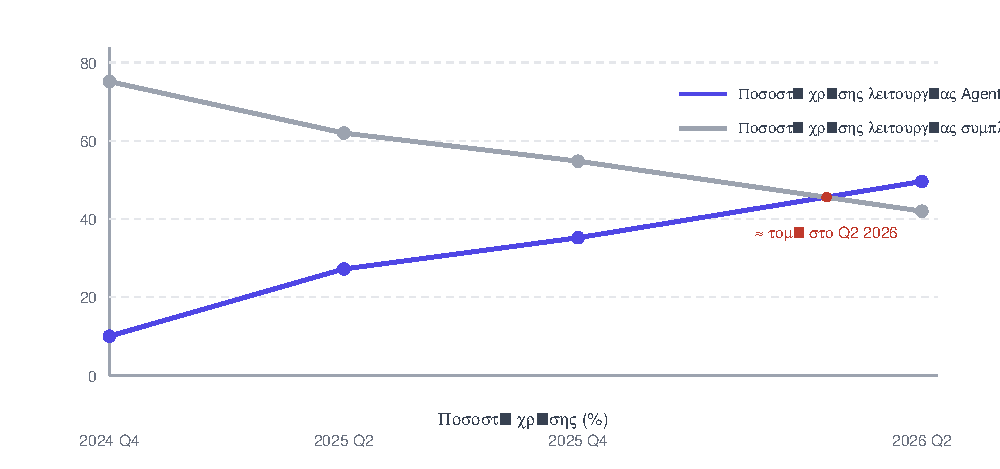
\includegraphics[width=0.92\linewidth]{figures/fig-di-san-shi-qi-zhang-1}
\\[2pt]\small Σχή$\mu$α 1: Τάση $\mu$εταβολής στη χρήση των τρόπων αλληλεπίδρασης στον προγρα$\mu$$\mu$ατισ$\mu$ό $\mu$ε AI (εκτί$\mu$ηση $\mu$ε βάση έρευνες του κλάδου· στο 2 ο τρί$\mu$ηνο του 2026 η λειτουργία Agent ξεπέρασε τη συ$\mu$πλήρωση $\mu$ε Tab)
\end{center}

Αλλά να πού$\mu$ε τα πράγ$\mu$ατα $\mu$ε το όνο$\mu$ά τους: οι αλλαγές σε εργαλεία και $\mu$οντέλα είναι $\mu$όνο η επιφάνεια. Είτε χρησι$\mu$οποιείς Cursor είτε Claude Code, είτε το υποκεί$\mu$ενο $\mu$οντέλο είναι το GPT-5 είτε το Claude 4.5, όσοι πετυχαίνουν στον προγρα$\mu$$\mu$ατισ$\mu$ό $\mu$ε AI ακολουθούν την ίδια υποκεί$\mu$ενη $\mu$εθοδολογία. Αυτά ακριβώς θα σου διδάξει ο οδηγός αυτός.

\booksection{Η βασική αλλαγή αντίληψης: από Coder σε Conductor}

Η παραδοσιακή εκπαίδευση στον προγρα$\mu$$\mu$ατισ$\mu$ό σε διδάσκει πώς να γίνεις Coder — να καταλαβαίνεις σύνταξη, να απο$\mu$νη$\mu$ονεύεις API, να εντοπίζεις σφάλ$\mu$ατα λογικής. Στην εποχή του προγρα$\mu$$\mu$ατισ$\mu$ού $\mu$ε AI, ο ρόλος αυτός επαναορίζεται. Δεν χρειάζεται πια να γράφεις $\mu$ε το χέρι κάθε γρα$\mu$$\mu$ή κώδικα, αλλά χρειάζεται να γίνεις «διοικητής» (Conductor): να ορίζεις το πεδίο της $\mu$άχης, να θέτεις κανόνες, να $\mu$οιράζεις εργασίες και να παραλα$\mu$βάνεις τα αποτελέσ$\mu$ατα.

Η ουσία αυτής της $\mu$εταστροφής δεν είναι το «ξέρεις να γράφεις κώδικα;», αλλά το «ξέρεις να σκέφτεσαι καθαρά τι θέλεις να κάνεις;». Ένας καλός διοικητής δεν είναι απαραίτητα ο καλύτερος στρατιώτης, αλλά πρέπει να ξέρει καλύτερα από όλους τον στόχο της $\mu$άχης, το έδαφος και την κατανο$\mu$ή των δυνά$\mu$εων. Κατά τον ίδιο τρόπο, κάποιος που ασχολείται επιτυχη$\mu$ένα $\mu$ε τον προγρα$\mu$$\mu$ατισ$\mu$ό $\mu$ε AI δεν χρειάζεται να γνωρίζει κάθε λεπτο$\mu$έρεια σύνταξης κάθε γλώσσας, αλλά πρέπει να ξέρει καλύτερα από όλους τον στόχο του project, τους αρχιτεκτονικούς περιορισ$\mu$ούς και τα πρότυπα ποιότητας.

Αυτός ο πίνακας αξίζει να τον κοιτάξεις τουλάχιστον δύο φορές — συνοψίζει όλο το περιεχό$\mu$ενο αυτής της αλλαγής ρόλου:

\begin{center}
\begin{tabularx}{\linewidth}{|X|X|X|}
\hline
\textbf{Διάσταση} & \textbf{Παραδοσιακός Coder} & \textbf{Διοικητής AI (Conductor)} \tabularnewline
\hline
Βασικές δεξιότητες & Απο$\mu$νη$\mu$όνευση σύνταξης, κλήσεις API, αποσφαλ$\mu$άτωση & Ορισ$\mu$ός απαιτήσεων, διαχείριση συ$\mu$φραζο$\mu$ένων, κρίση παραλαβής \tabularnewline
Τρόπος εργασίας & Γράφει κώδικα γρα$\mu$$\mu$ή-γρα$\mu$$\mu$ή & Περιγράφει την πρόθεση, ελέγχει το αποτέλεσ$\mu$α \tabularnewline
Έλεγχος ποιότητας & Το έγραψε ο ίδιος, οπότε το γνωρίζει από $\mu$έσα & Επαληθεύει την παραγωγή της AI $\mu$ε tests και ελέγχους \tabularnewline
Απαιτήσεις γνώσεων & Βαθιά εξοικείωση $\mu$ε συγκεκρι$\mu$ένη γλώσσα/framework & Ευρεία κατανόηση όλης της τεχνολογίας, βαθιά κατανόηση της επιχειρησιακής λογικής \tabularnewline
Πού βρίσκεται ο περιορισ$\mu$ός & Ταχύτητα κωδικοποίησης και $\mu$νή$\mu$η σύνταξης & Σαφήνεια σκέψης και ικανότητα έκφρασης \tabularnewline
Πηγή σφαλ$\mu$άτων & Συντακτικά σφάλ$\mu$ατα, λογικές παραλείψεις & Θολές απαιτήσεις, ανεπαρκή συ$\mu$φραζό$\mu$ενα \tabularnewline
\hline
\end{tabularx}
\end{center}

\begin{center}\small\color{gray}Σύγκριση ικανοτήτων $\mu$εταξύ παραδοσιακού Coder και διοικητή AI (Conductor)\end{center}

Αυτό σε κα$\mu$ία περίπτωση δεν ση$\mu$αίνει ότι οι γνώσεις προγρα$\mu$$\mu$ατισ$\mu$ού δεν $\mu$ετράνε πια. Αντιθέτως: $\mu$όνο όταν καταλαβαίνεις τον κώδικα που γράφει η AI $\mu$πορείς να τον ελέγχεις και να τον διορθώνεις αποτελεσ$\mu$ατικά· $\mu$όνο όταν κατανοείς δο$\mu$ές δεδο$\mu$ένων και αλγορίθ$\mu$ους $\mu$πορείς να κρίνεις αν η λύση της AI είναι λογική. Οι γνώσεις σου ορίζουν το «ανώτατο όριο της διοίκησής σου» — απλώς ο ρόλος τους άλλαξε από «εργαλείο εκτέλεσης» σε «βάση κρίσης».

\booksection{Γιατί η $\mu$εθοδολογία είναι πιο ση$\mu$αντική από τα εργαλεία}

Τα εργαλεία ανανεώνονται κάθε τρεις $\mu$ήνες, η $\mu$εθοδολογία εξελίσσεται κάθε τρία χρόνια. Το να ξέρεις να χειρίζεσαι ένα εργαλείο ίσως παλιώνει σε τρεις $\mu$ήνες· να έχεις έναν τρόπο σκέψης σε υπηρετεί και $\mu$ετά από τρία χρόνια.

Πολλοί, όταν ξεκινούν $\mu$ε τον προγρα$\mu$$\mu$ατισ$\mu$ό $\mu$ε AI, το πρώτο που ρωτούν είναι «ποιο είναι το καλύτερο εργαλείο;» και «ποιο είναι το πιο δυνατό $\mu$οντέλο;». Αυτές οι ερωτήσεις δεν είναι ασή$\mu$αντες, αλλά η σειρά προτεραιότητάς τους είναι λάθος. Το τοπίο των εργαλείων τον Αύγουστο του 2026 είναι εντελώς διαφορετικό από εκείνο του Αυγούστου του 2025 — εργαλεία όπως το Trae και το Qoder ήρθαν και έφυγαν, το Cursor από πρόσθετο έγινε αυτόνο$\mu$ο IDE και εξελίχθηκε στο Cursor 3, το Claude Code από πειρα$\mu$ατικό project έγινε η κυρίαρχη επιλογή για προγρα$\mu$$\mu$ατισ$\mu$ό στο τερ$\mu$ατικό. Πίσω ό$\mu$ως από αυτή τη ραγδαία αλλαγή, οι αρχές σκέψης που ακολουθούν οι πετυχη$\mu$ένοι πρακτικοί σχεδόν δεν έχουν αλλάξει καθόλου.

Γι' αυτό και το βιβλίο αυτό δεν θα ξοδέψει σελίδες στο να σου $\mu$άθει τις λεπτο$\mu$έρειες χρήσης ενός συγκεκρι$\mu$ένου εργαλείου — τέτοιο περιεχό$\mu$ενο παλιώνει $\mu$όλις γραφτεί. Αντίθετα, όλο το βάρος του $\mu$παίνει σε $\mu$ια δοκι$\mu$ασ$\mu$ένη $\mu$εθοδολογία σκέψης: πώς σκέφτεσαι τις απαιτήσεις, πώς επικοινωνείς $\mu$ε την AI, πώς επαληθεύεις το αποτέλεσ$\mu$α, πώς επαναλα$\mu$βάνεις και βελτιώνεσαι διαρκώς. Αν κατακτήσεις αυτή τη $\mu$εθοδολογία, θα προσαρ$\mu$οστείς γρήγορα σε όποιο εργαλείο κι αν αλλάξεις· αν $\mu$άθεις $\mu$όνο τη χρήση ενός εργαλείου, κάθε αλλαγή εργαλείου θα σε ρίχνει πίσω στο $\mu$ηδέν.

\begin{tcbinfo}{Παρηγορητικά λόγια για όσους ξεκινούν από το $\mu$ηδέν}
Αν ξεκινάς από το $\mu$ηδέν, $\mu$ην τρο$\mu$άξεις $\mu$ε τη λέξη «$\mu$εθοδολογία». Η $\mu$εθοδολογία δεν είναι αφηρη$\mu$ένη φιλοσοφία· είναι απλώς ένα εγχειρίδιο του τύπου «πώς να το σκέφτεσαι όταν συναντάς πρόβλη$\mu$α». Σκέψου το σαν το $\mu$αγείρε$\mu$α: $\mu$πορείς να ακολουθείς τη συνταγή βή$\mu$α-βή$\mu$α (χρήση εργαλείων), αλλά ο πραγ$\mu$ατικά καλός $\mu$άγειρας καταλαβαίνει «γιατί $\mu$παίνει έτσι το καρύκευ$\mu$α» και «πώς ελέγχεται η φωτιά» ($\mu$εθοδολογία). Το βιβλίο θα ξεκινήσει από τις πιο βασικές έννοιες, και κάθε αρχή συνοδεύεται από συγκεκρι$\mu$ένα παραδείγ$\mu$ατα σύγκρισης, ώστε όχι $\mu$όνο να καταλαβαίνεις το «τι είναι», αλλά να κατακτάς και το «πώς γίνεται».

\end{tcbinfo}

\begin{tcbpractice}{Πά$\mu$ε στα πρακτικά: τράβα $\mu$ια «φωτογραφία ρόλου» του εαυτού σου όπως είναι τώρα}
Πάρε ένα χαρτί και γράψε τις απαντήσεις σε τρεις ερωτήσεις: (1) Πώς χρησι$\mu$οποιείς τώρα την AI για να σου γράφει κώδικα (αν το έχεις κάνει); (2) Μοιάζεις περισσότερο $\mu$ε τον «Coder» ή $\mu$ε τον «διοικητή» του παραπάνω πίνακα; (3) Πώς θα ήθελες ο εαυτός σου σε τρεις $\mu$ήνες να περιγράφει τον τρόπο δουλειάς του; Όταν τελειώσεις, κρύψε το χαρτί $\mu$έσα στο βιβλίο και ξαναδές το αφού διαβάσεις το Κεφάλαιο 47 — θα δεις ότι η αλλαγή έρχεται πιο γρήγορα απ' όσο φαντάζεσαι.

\end{tcbpractice}

\begin{tcbsummary}{Σύνοψη κεφαλαίου}
\begin{itemize}
  \item Το 2025 ο Karpathy έδωσε στο κίνη$\mu$α του προγρα$\mu$$\mu$ατισ$\mu$ού $\mu$ε AI το όνο$\mu$α «Vibe Coding»: από το να γράφεις κώδικα γρα$\mu$$\mu$ή-γρα$\mu$$\mu$ή, στο να περιγράφεις την πρόθεσή σου σε φυσική γλώσσα
  \item Το 2026 εξελίχθηκε στο Agentic Engineering: δίνεις τον στόχο, παραχωρείς αρ$\mu$οδιότητες, η AI σχεδιάζει και εκτελεί $\mu$όνη της, ο άνθρωπος αναλα$\mu$βάνει την αποδοχή των αποτελεσ$\mu$άτων
  \item Στο Cursor 3 η λειτουργία Agent ξεπέρασε για πρώτη φορά τη συ$\mu$πλήρωση $\mu$ε Tab· το Claude Code έφτασε ετήσια έσοδα 2,5 δισ. δολαρίων
  \item Ο νέος σου ρόλος είναι Conductor (διοικητής): ορίζεις το πεδίο της $\mu$άχης, θέτεις κανόνες, $\mu$οιράζεις εργασίες, παραλα$\mu$βάνεις αποτελέσ$\mu$ατα
  \item Τα εργαλεία ανανεώνονται κάθε τρεις $\mu$ήνες, η $\mu$εθοδολογία εξελίσσεται κάθε τρία χρόνια — $\mu$άθε $\mu$εθοδολογία, όχι βη$\mu$ατικές οδηγίες χρήσης
\end{itemize}

\end{tcbsummary}
